\chapter{Forze conservative e stabilità}

\section{Forze conservative}
\begin{definition}{}[Forze conservative]
Dico che una forza è posizionale se
\[
\underline{f}=\underline{f}(\underline{x}).
\]
Se
\[
\underline{f}(\underline{x})=-\nabla V,
\]
dove
\[
V:\mathbb{R}^3\to\mathbb{R},
\qquad
\underline{x}\mapsto V(\underline{x}),
\]
si dice energia potenziale, allora diciamo che \(\underline{f}\) è conservativa.
\end{definition}

\begin{oss}{}
Spesso sui libri di matematica è introdotta la funzione potenziale
\[
U(\underline{x})=-V(\underline{x})
\]
tale che
\[
\underline{f}=\nabla U.
\]
\end{oss}

\begin{oss}{}
Condizione necessaria per cui \(\underline{f}\) posizionale sia conservativa è che
\[
\nabla\times \underline{f}=\underline{0},
\]
perché
\[
\nabla\times(\nabla U)=\underline{0}.
\]
In un dominio semplicemente connesso tale condizione è anche sufficiente.
\end{oss}

\begin{oss}{}
Tutte le forze in \(\mathbb{R}\) sono conservative. Non è vero in dimensione superiore.

Ad esempio,
\[
\underline{f}(x,y,z)
=
\begin{pmatrix}
x^2y+z\\
2xy\\
xy^2
\end{pmatrix}.
\]
Allora
\[
\nabla\times\underline{f}\neq \underline{0},
\]
infatti
\[
\left(\nabla\times\underline{f}\right)_z
=
x^2-2y\neq 0.
\]
\end{oss}

\begin{oss}{}
L'energia potenziale è sempre definita a meno di una costante:
\[
\underline{f}
=
-\nabla V
=
-\nabla \hat{V},
\]
con
\[
\hat{V}=V+c,
\qquad c\in\mathbb{R}.
\]
\end{oss}

\begin{oss}{}
Essendo
\[
\underline{f}=-\nabla V,
\]
allora
\[
\underline{f}=\underline{0}
\quad\Longrightarrow\quad
\nabla V=\underline{0}.
\]
Ovvero, i punti di equilibrio sono i punti stazionari di \(V\).
\end{oss}

\begin{example}{}[Forza peso]
Consideriamo la forza peso
\[
\underline{f}=-mg\hat{k},
\]
con
\[
V:\mathbb{R}^3\to\mathbb{R}.
\]
Poiché
\[
\underline{f}=-\nabla V,
\]
si ha
\[
-\nabla V=
\left\{
\begin{array}{l}
-\dfrac{\partial V}{\partial x}=0,\\[2mm]
-\dfrac{\partial V}{\partial y}=0,\\[2mm]
-\dfrac{\partial V}{\partial z}=-mg.
\end{array}
\right.
\]
Da cui
\[
V=mgz+c.
\]

Fisicamente la costante è legata all'arbitrarietà di fissare l'asse \(z\).
\end{example}

\begin{example}{}[Forza elastica lineare nello spazio]
    Si consideri una forza elastica lineare nello spazio.
\begin{center}
\begin{tikzpicture}[
    x=1cm,
    y=1cm,
    >=Latex,
    line cap=round,
    line join=round,
    every node/.style={font=\small}
]

% punti
\coordinate (A) at (0,0);
\coordinate (M) at (2.2,1.2);

% punto fisso A
\draw[black, line width=1pt] ($(A)+(-0.10,-0.10)$) -- ($(A)+(0.10,0.10)$);
\draw[black, line width=1pt] ($(A)+(-0.10,0.10)$) -- ($(A)+(0.10,-0.10)$);
\node[below left] at (A) {$A$};

% molla
\draw[yellow!80!orange!90!black, line width=1.3pt] (A) -- ++(0.18,0.10);
\draw[yellow!80!orange!90!black, line width=1.3pt, smooth, samples=120, domain=0:1.75]
plot ({0.18 + \x*1.05},{0.10 + \x*0.60 + 0.12*sin(deg(\x*15))});
\draw[yellow!80!orange!90!black, line width=1.3pt] (2.02,1.10) -- (M);

% massa
\fill[black] (M) circle (1.7pt);
\node[above right] at (M) {$m$};

% forza
\draw[red!80!black, line width=1.4pt, ->] ($(M)+(-0.02,-0.02)$) -- ++(-0.55,-0.30);
\node[red!80!black, below] at ($(M)+(-0.30,-0.38)$) {$\underline{f}$};

\end{tikzpicture}
\end{center}

 In tal caso
\[
\underline{f}
=
-k\left(\underline{x}-\underline{x}_A\right)
=
-k
\begin{pmatrix}
x-x_A\\
y-y_A\\
z-z_A
\end{pmatrix}
=
-\nabla V.
\]

Equivalentemente,
\[
\nabla V
=
k
\begin{pmatrix}
x-x_A\\
0\\
0
\end{pmatrix}
+
k
\begin{pmatrix}
0\\
y-y_A\\
0
\end{pmatrix}
+
k
\begin{pmatrix}
0\\
0\\
z-z_A
\end{pmatrix}.
\]

Da cui si ottiene
\[
V(\underline{X})
=
\frac{1}{2}k(x-x_A)^2
+
\frac{1}{2}k(y-y_A)^2
+
\frac{1}{2}k(z-z_A)^2.
\]

In una dimensione:

\begin{center}
\begin{tikzpicture}[
    x=1cm,
    y=1cm,
    >=Latex,
    line cap=round,
    line join=round,
    every node/.style={font=\small}
]

% asse
\draw[black, line width=1pt] (0,0) -- (4.8,0);

% punto O e vincolo a sinistra
\draw[black, line width=1pt] (0.25,-0.18) -- (0.25,0.18);
\node[below] at (0.25,-0.18) {$O$};

% molla
\draw[yellow!80!orange!90!black, line width=1.3pt] (0.25,0) -- (0.55,0);
\draw[yellow!80!orange!90!black, line width=1.3pt, smooth, samples=120, domain=0.55:3.10]
plot (\x,{0.12*sin(deg((\x-0.55)*18))});
\draw[yellow!80!orange!90!black, line width=1.3pt] (3.10,0) -- (3.45,0);

% massa
\fill[black] (3.65,0) circle (1.9pt);
\node[below] at (3.65,-0.05) {$x$};

% forza
\draw[red!80!black, line width=1.4pt, ->] (3.45,0.14) -- ++(-1.05,0);
\node[red!80!black, above] at (2.90,0.20) {$-Kx\,\hat{\imath}$};

\end{tikzpicture}
\end{center}

\[
\underline{f}_1=-kx\,\hat{\imath}
\qquad \Longrightarrow \qquad
V=\frac{1}{2}kx^2.
\]
\end{example}

\begin{theorem}{}
    Le forze conservative preservano l'energia totale (cinetica + potenziale).
\end{theorem}

\begin{proof}
Consideriamo un punto materiale
\[
\underline{x}(t),
\qquad
\underline{v}=\dot{\underline{x}}(t),
\qquad
\underline{a}=\ddot{\underline{x}}(t).
\]
Per la seconda legge della dinamica si ha
\[
\underline{f}=m\ddot{\underline{x}}.
\]

Moltiplicando scalarmente per \(\dot{\underline{x}}\), otteniamo
\[
m\ddot{\underline{x}}\cdot \dot{\underline{x}}
=
\underline{f}\cdot \dot{\underline{x}}.
\]
Supponiamo che \(\underline{f}\) sia conservativa, cioè
\[
\underline{f}=-\nabla V.
\]
Allora
\[
m\ddot{\underline{x}}\cdot \dot{\underline{x}}
=
-\nabla V\cdot \dot{\underline{x}}.
\]

Esplicitamente,
\[
-\nabla V\cdot \dot{\underline{x}}
=
-
\begin{pmatrix}
\dfrac{\partial V}{\partial x}\\[2mm]
\dfrac{\partial V}{\partial y}\\[2mm]
\dfrac{\partial V}{\partial z}
\end{pmatrix}
\cdot
\begin{pmatrix}
\dot{x}\\[1mm]
\dot{y}\\[1mm]
\dot{z}
\end{pmatrix}.
\]
Per la regola della catena,
\[
\nabla V\cdot \dot{\underline{x}}
=
\frac{dV}{dt}.
\]
Quindi
\[
m\ddot{\underline{x}}\cdot \dot{\underline{x}}
=
-\frac{dV}{dt}.
\]

Ora
\[
\ddot{\underline{x}}\cdot \dot{\underline{x}}
=
\frac{1}{2}\frac{d}{dt}
\left(
\dot{\underline{x}}\cdot \dot{\underline{x}}
\right),
\]
perciò
\[
m\frac{d}{dt}
\left(
\frac{1}{2}\dot{\underline{x}}\cdot \dot{\underline{x}}
\right)
=
-\frac{dV}{dt}.
\]
Dunque
\[
\frac{dT}{dt}
=
-\frac{dV}{dt},
\]
dove
\[
T=
\frac{1}{2}m\dot{\underline{x}}\cdot \dot{\underline{x}}
\]
è l'energia cinetica.

Pertanto
\[
\frac{d}{dt}(T+V)=0,
\]
e quindi
\[
T+V=\text{cost}.
\]
\end{proof}


\begin{example}{}[Oscillatore armonico]
    Studiamo l'energia di un oscillatore armonico.
\begin{figure}
\centering
\begin{tikzpicture}[scale=1,>=Latex]

% Parete
\draw[line width=1pt] (0,0) -- (0,1.5);

% Molla
\draw[red!80!black,line width=1pt] (0.08,0.75) -- (0.25,0.75);
\draw[red!80!black,line width=1pt]
(0.25,0.75)
-- (0.35,0.85)
-- (0.45,0.65)
-- (0.55,0.85)
-- (0.65,0.65)
-- (0.75,0.85)
-- (0.85,0.65)
-- (0.95,0.85)
-- (1.05,0.65)
-- (1.15,0.85)
-- (1.25,0.65)
-- (1.35,0.85)
-- (1.45,0.65)
-- (1.55,0.85)
-- (1.65,0.65)
-- (1.75,0.75);

% asta finale e massa
\draw[line width=1pt] (1.75,0.75) -- (1.95,0.75);
\fill (0.08,0.75) circle (1.6pt);
\fill (1.95,0.75) circle (1.6pt);

% forza
\draw[->,line width=1pt] (1.55,1.15) -- (1.05,1.15);
\node[above] at (1.30,1.18) {$-k \underline{x}\,\hat{\imath}$};

\end{tikzpicture}
\end{figure}

\[
T=\frac{m\dot{x}^{2}}{2},
\qquad
V=\frac{kx^{2}}{2},
\]
per cui
\[
E=\frac{m\dot{x}^{2}}{2}+\frac{kx^{2}}{2}=\text{cost.}
\]

Nel tempo
\[
x(t)=A\cos(\omega t+\varphi),
\qquad
\omega=\sqrt{\frac{k}{m}},
\]
dove \(A\) e \(\varphi\) dipendono dalle c.i.

\begin{figure}
\centering
\begin{tikzpicture}[scale=1,>=Latex]

% Assi
\draw[->,line width=1pt] (0,-1.4) -- (0,1.4);
\draw[->,line width=1pt] (0,0) -- (4.3,0);
\node[right] at (4.3,0) {$t$};

% Curve
\draw[green!60!black,line width=1pt,samples=200,smooth,domain=0:3.4]
plot (\x,{0.8*cos(deg(2.1*\x-0.2))});
\draw[red!80!black,line width=1pt,samples=200,smooth,domain=0:3.4]
plot (\x,{0.8*sin(deg(2.1*\x))});

% punti
\fill[green!60!black] (0,0.78) circle (1.5pt);
\fill[red!80!black] (0,0) circle (1.5pt);
\fill[green!60!black] ({pi/2/2.1+0.1},{0}) circle (1.5pt);
\fill[red!80!black] ({pi/2/2.1},{0.8}) circle (1.5pt);
\fill[red!80!black] ({pi/2/2.1+pi/2/2.1},{-0.8}) circle (1.5pt);
\fill[red!80!black] (3.3,0) circle (1.5pt);

% etichette
\node[green!60!black,right] at (3.0,0.55) {$x(t)$};
\node[red!80!black,below] at (2.9,-0.55) {$\dot{x}(t)$};

\end{tikzpicture}
\end{figure}

Alternativamente, nel piano delle fasi \((x(t),\dot{x}(t))\), la relazione
\[
\frac{m}{2E}\dot{x}^{2}+\frac{k}{2E}x^{2}=1
\]
descrive un'ellisse centrata nell'origine. Tale ellisse è espressa in forma parametrica come curva nel piano delle fasi da
\[
(x(t),\dot{x}(t)).
\]

\begin{figure}
\centering
\begin{tikzpicture}[scale=1,>=Latex]

% Assi
\draw[->,line width=1pt] (-3.8,0) -- (3.9,0);
\draw[->,line width=1pt] (0,-2.8) -- (0,2.8);
\node[right] at (3.9,0) {$x$};
\node[above] at (0,2.8) {$\dot{x}$};

% Parametri ellissi
\def\aext{3.0}
\def\bext{2.0}
\def\aint{1.8}
\def\bint{1.0}

% Ellissi
\draw[line width=1pt] (0,0) ellipse (3.0 and 2.0);
\draw[line width=1pt] (0,0) ellipse (1.8 and 1.0);

% Punto massimo di velocità sull'ellisse interna
\fill (0,\bint) circle (1.5pt);
\node[right] at (0.08,\bint+0.08) {$\dot{x}_{\max}$};

% Etichetta x_max
\node[below] at (\aint,-0.06) {$x_{\max}$};

% Frecce tangenti all'ellisse esterna (moto orario)
\draw[->,line width=0.8pt]
({\aext*cos(140)},{\bext*sin(140)})
--
({\aext*cos(128)},{\bext*sin(128)});

\draw[->,line width=0.8pt]
({\aext*cos(95)},{\bext*sin(95)})
--
({\aext*cos(83)},{\bext*sin(83)});

\draw[->,line width=0.8pt]
({\aext*cos(40)},{\bext*sin(40)})
--
({\aext*cos(28)},{\bext*sin(28)});

\draw[->,line width=0.8pt]
({\aext*cos(-10)},{\bext*sin(-10)})
--
({\aext*cos(-22)},{\bext*sin(-22)});

\draw[->,line width=0.8pt]
({\aext*cos(-55)},{\bext*sin(-55)})
--
({\aext*cos(-67)},{\bext*sin(-67)});

\draw[->,line width=0.8pt]
({\aext*cos(-115)},{\bext*sin(-115)})
--
({\aext*cos(-127)},{\bext*sin(-127)});

% Frecce tangenti all'ellisse interna (moto orario)
\draw[->,line width=0.8pt]
({\aint*cos(145)},{\bint*sin(145)})
--
({\aint*cos(132)},{\bint*sin(132)});

\draw[->,line width=0.8pt]
({\aint*cos(85)},{\bint*sin(85)})
--
({\aint*cos(70)},{\bint*sin(70)});

\draw[->,line width=0.8pt]
({\aint*cos(25)},{\bint*sin(25)})
--
({\aint*cos(10)},{\bint*sin(10)});

\draw[->,line width=0.8pt]
({\aint*cos(-20)},{\bint*sin(-20)})
--
({\aint*cos(-35)},{\bint*sin(-35)});

\draw[->,line width=0.8pt]
({\aint*cos(-95)},{\bint*sin(-95)})
--
({\aint*cos(-110)},{\bint*sin(-110)});

\draw[->,line width=0.8pt]
({\aint*cos(-155)},{\bint*sin(-155)})
--
({\aint*cos(-170)},{\bint*sin(-170)});

% Freccia rossa uscente dall'ellisse interna verso quella esterna
\coordinate (Pin)  at ({\aint*cos(40)},{\bint*sin(40)});
\coordinate (Pout) at ({\aext*cos(40)},{\bext*sin(40)});
\draw[->,red!80!black,line width=1pt] (Pin) -- (Pout);
\node[red!80!black,right] at ($(Pin)!0.55!(Pout)+(0.10,0.05)$) {$E$};

\end{tikzpicture}
\end{figure}

Possiamo notare che la velocità massima
\[
\dot{x}_{\max}=\sqrt{\frac{2E}{m}}
\]
è assunta in corrispondenza di \(x=0\), e la posizione massima
\[
x_{\max}=\sqrt{\frac{2E}{k}}
\]
è assunta in corrispondenza di \(\dot{x}=0\). Inoltre, aumentando \(E\), l'orbita si allarga, ovvero possiamo raggiungere velocità e posizioni maggiori.
\end{example}



\begin{example}{}[Pendolo semplice nel piano delle fasi]
    Studiamo le configurazioni energetiche del pendolo semplice.
    \begin{center}
        \begin{tikzpicture}[
    x=1cm,
    y=1cm,
    >=Latex,
    line cap=round,
    line join=round,
    every node/.style={font=\small}
]

% Coordinate
\coordinate (O) at (0,0);
\coordinate (P) at (2.15,-2.10);

% Retta z = 0
\draw[green!60!black, line width=1.2pt] (-2.00,0) -- (4.80,0);
\node[green!60!black, right] at (5.05,0.08) {$z=0$};

% Verticale di riferimento
\draw[black, line width=1.4pt] (O) -- (0,-3.15);

% Punto fisso
\fill[black] (O) circle (2.4pt);

% Asta
\draw[black, line width=1.5pt] (O) -- (P);
\node[above right] at ($(O)!0.42!(P)$) { $l$};

% Massa
\fill[black] (P) circle (2.4pt);
\node[right] at ($(P)+(0.12,0.02)$) { $m$};

% Angolo theta
\draw[black, line width=1.1pt, ->]
(0,-1.20) arc[start angle=-90,end angle=-45,radius=1.20];
\node at (0.55,-1.45) { $\theta$};

% Freccia peso
\draw[red!80!black, line width=1.5pt, ->] (P) -- ++(0,-1.05);
\node[red!80!black, right] at ($(P)+(0.48,-0.68)$) { $m\underline{g}$};

% Piccolo arco di traiettoria
\draw[black, line width=1.3pt]
($(P)+(-0.78,-0.90)$)
.. controls ($(P)+(-0.15,-0.48)$) and ($(P)+(0.30,0.15)$)
.. ($(P)+(0.42,0.65)$);

\end{tikzpicture}
    \end{center}

Si ha
\[
T
=
\frac{m\dot{x}^{2}}{2}
=
\frac{m}{2}\left(\ell\dot{\theta}\right)^2,
\qquad
V
=
-mg\ell\cos\theta.
\]
Quindi
\[
E
=
\frac{m}{2}\left(\ell\dot{\theta}\right)^2
-
mg\ell\cos\theta.
\]

Vogliamo studiare il luogo geometrico descritto nel piano delle fasi, come nell'esercizio precedente. Risulta complicato globalmente. Studiamo cosa succede se \(\theta\) è piccolo.

Per
\[
\theta\to 0
\]
si ha
\[
\cos\theta
\simeq
1-\frac{\theta^2}{2}.
\]
Allora
\[
E
=
\frac{m}{2}\left(\ell\dot{\theta}\right)^2
-
mg\ell
\left(
1-\frac{\theta^2}{2}
\right),
\]
da cui
\[
E+mg\ell
=
\frac{m\ell^2}{2}\dot{\theta}^{\,2}
+
\frac{mg\ell}{2}\theta^2.
\]
Quindi
\[
1
=
\frac{m\ell^2}{2E+2mg\ell}\dot{\theta}^{\,2}
+
\frac{mg\ell}{2E+2mg\ell}\theta^2.
\]

Per \(\theta\to 0\) ho quindi di nuovo un'ellisse.

\begin{center}
\begin{tikzpicture}[
    x=1cm,
    y=1cm,
    >=Latex,
    line cap=round,
    line join=round,
    every node/.style={font=\small}
]

% Assi
\draw[->, line width=1pt] (-2.0,0) -- (2.3,0) node[right] {$\theta$};
\draw[->, line width=1pt] (0,-1.25) -- (0,1.45) node[above] {$\dot{\theta}$};

% Ellisse
\draw[black, line width=1.1pt] (0,0) ellipse (1.15 and 0.42);

% Tacche e label
\draw[line width=0.9pt] (-1.15,-0.10) -- (-1.15,0.10);
\draw[line width=0.9pt] (1.15,-0.10) -- (1.15,0.10);

\node[below] at (-1.15,-0.08) {$-\varepsilon$};
\node[below] at (1.15,-0.08) {$\varepsilon$};
\node[below right] at (0,0) {$0$};

\node[right] at (2.65,0.15) {$\varepsilon\ll 1$};

\end{tikzpicture}
\end{center}

Possiamo fare lo stesso per
\[
\theta\to \pi.
\]
In questo caso
\[
\cos\theta
=
-1
+
\frac{1}{2}(\theta-\pi)^2
+
o\!\left((\theta-\pi)^2\right),
\qquad
\theta\to \pi.
\]
Allora
\[
E
=
\frac{m\ell^2}{2}\dot{\theta}^{\,2}
-
mg\ell
\left(
-1+\frac{1}{2}(\theta-\pi)^2
\right).
\]

Poniamo
\[
\hat{\theta}
=
\theta-\pi.
\]
Si ha
\[
E
=
\frac{m\ell^2}{2}\dot{\hat{\theta}}^{\,2}
-
mg\ell
\left(
-1+\frac{1}{2}\hat{\theta}^{\,2}
\right),
\]
cioè
\[
E-mg\ell
=
\frac{m\ell^2}{2}\dot{\hat{\theta}}^{\,2}
-
\frac{mg\ell}{2}\hat{\theta}^{\,2}.
\]
Quindi
\[
1
=
\frac{m\ell^2}{2E-2mg\ell}\dot{\hat{\theta}}^{\,2}
-
\frac{mg\ell}{2E-2mg\ell}\hat{\theta}^{\,2}.
\]

Ovvero otteniamo un'iperbole.

\begin{center}
\begin{tikzpicture}[
    x=1cm,
    y=1cm,
    >=Latex,
    line cap=round,
    line join=round,
    every node/.style={font=\small}
]

% Assi
\draw[->, line width=1pt] (-2.3,0) -- (2.5,0) node[right] {$\hat{\theta}$};
\draw[->, line width=1pt] (0,-2.2) -- (0,2.35) node[above] {$\dot{\hat{\theta}}$};

% Iperbole: rami verticali
\draw[black, line width=1.1pt, smooth, samples=120, domain=-1.35:1.35]
plot (\x,{0.75*sqrt(1 + 1.15*\x*\x)});

\draw[black, line width=1.1pt, smooth, samples=120, domain=-1.35:1.35]
plot (\x,{-0.75*sqrt(1 + 1.15*\x*\x)});

% Piccole frecce sui rami
\draw[->, line width=0.9pt] (-0.80,1.00) -- (-0.55,0.88);
\draw[->, line width=0.9pt] (0.55,0.88) -- (0.80,1.00);

\draw[->, line width=0.9pt] (-0.55,-0.88) -- (-0.80,-1.00);
\draw[->, line width=0.9pt] (0.80,-1.00) -- (0.55,-0.88);

\end{tikzpicture}
\end{center}

Notiamo che non per tutte le configurazioni d'energia \(\theta=\pi\) è una
posizione raggiungibile. L'energia potenziale è massima quando la cinetica è
nulla. La minima energia che dobbiamo dare per arrivare a \(\theta=\pi\) è
\[
E
=
-mg\ell\cos\pi
=
mg\ell.
\]

Se plottiamo la relazione
\[
E
=
\frac{m}{2}\left(\ell\dot{\theta}\right)^2
-
mg\ell\cos\theta
\]
con
\[
m=\ell=1
\]
per diversi livelli energetici, otteniamo

\begin{center}
    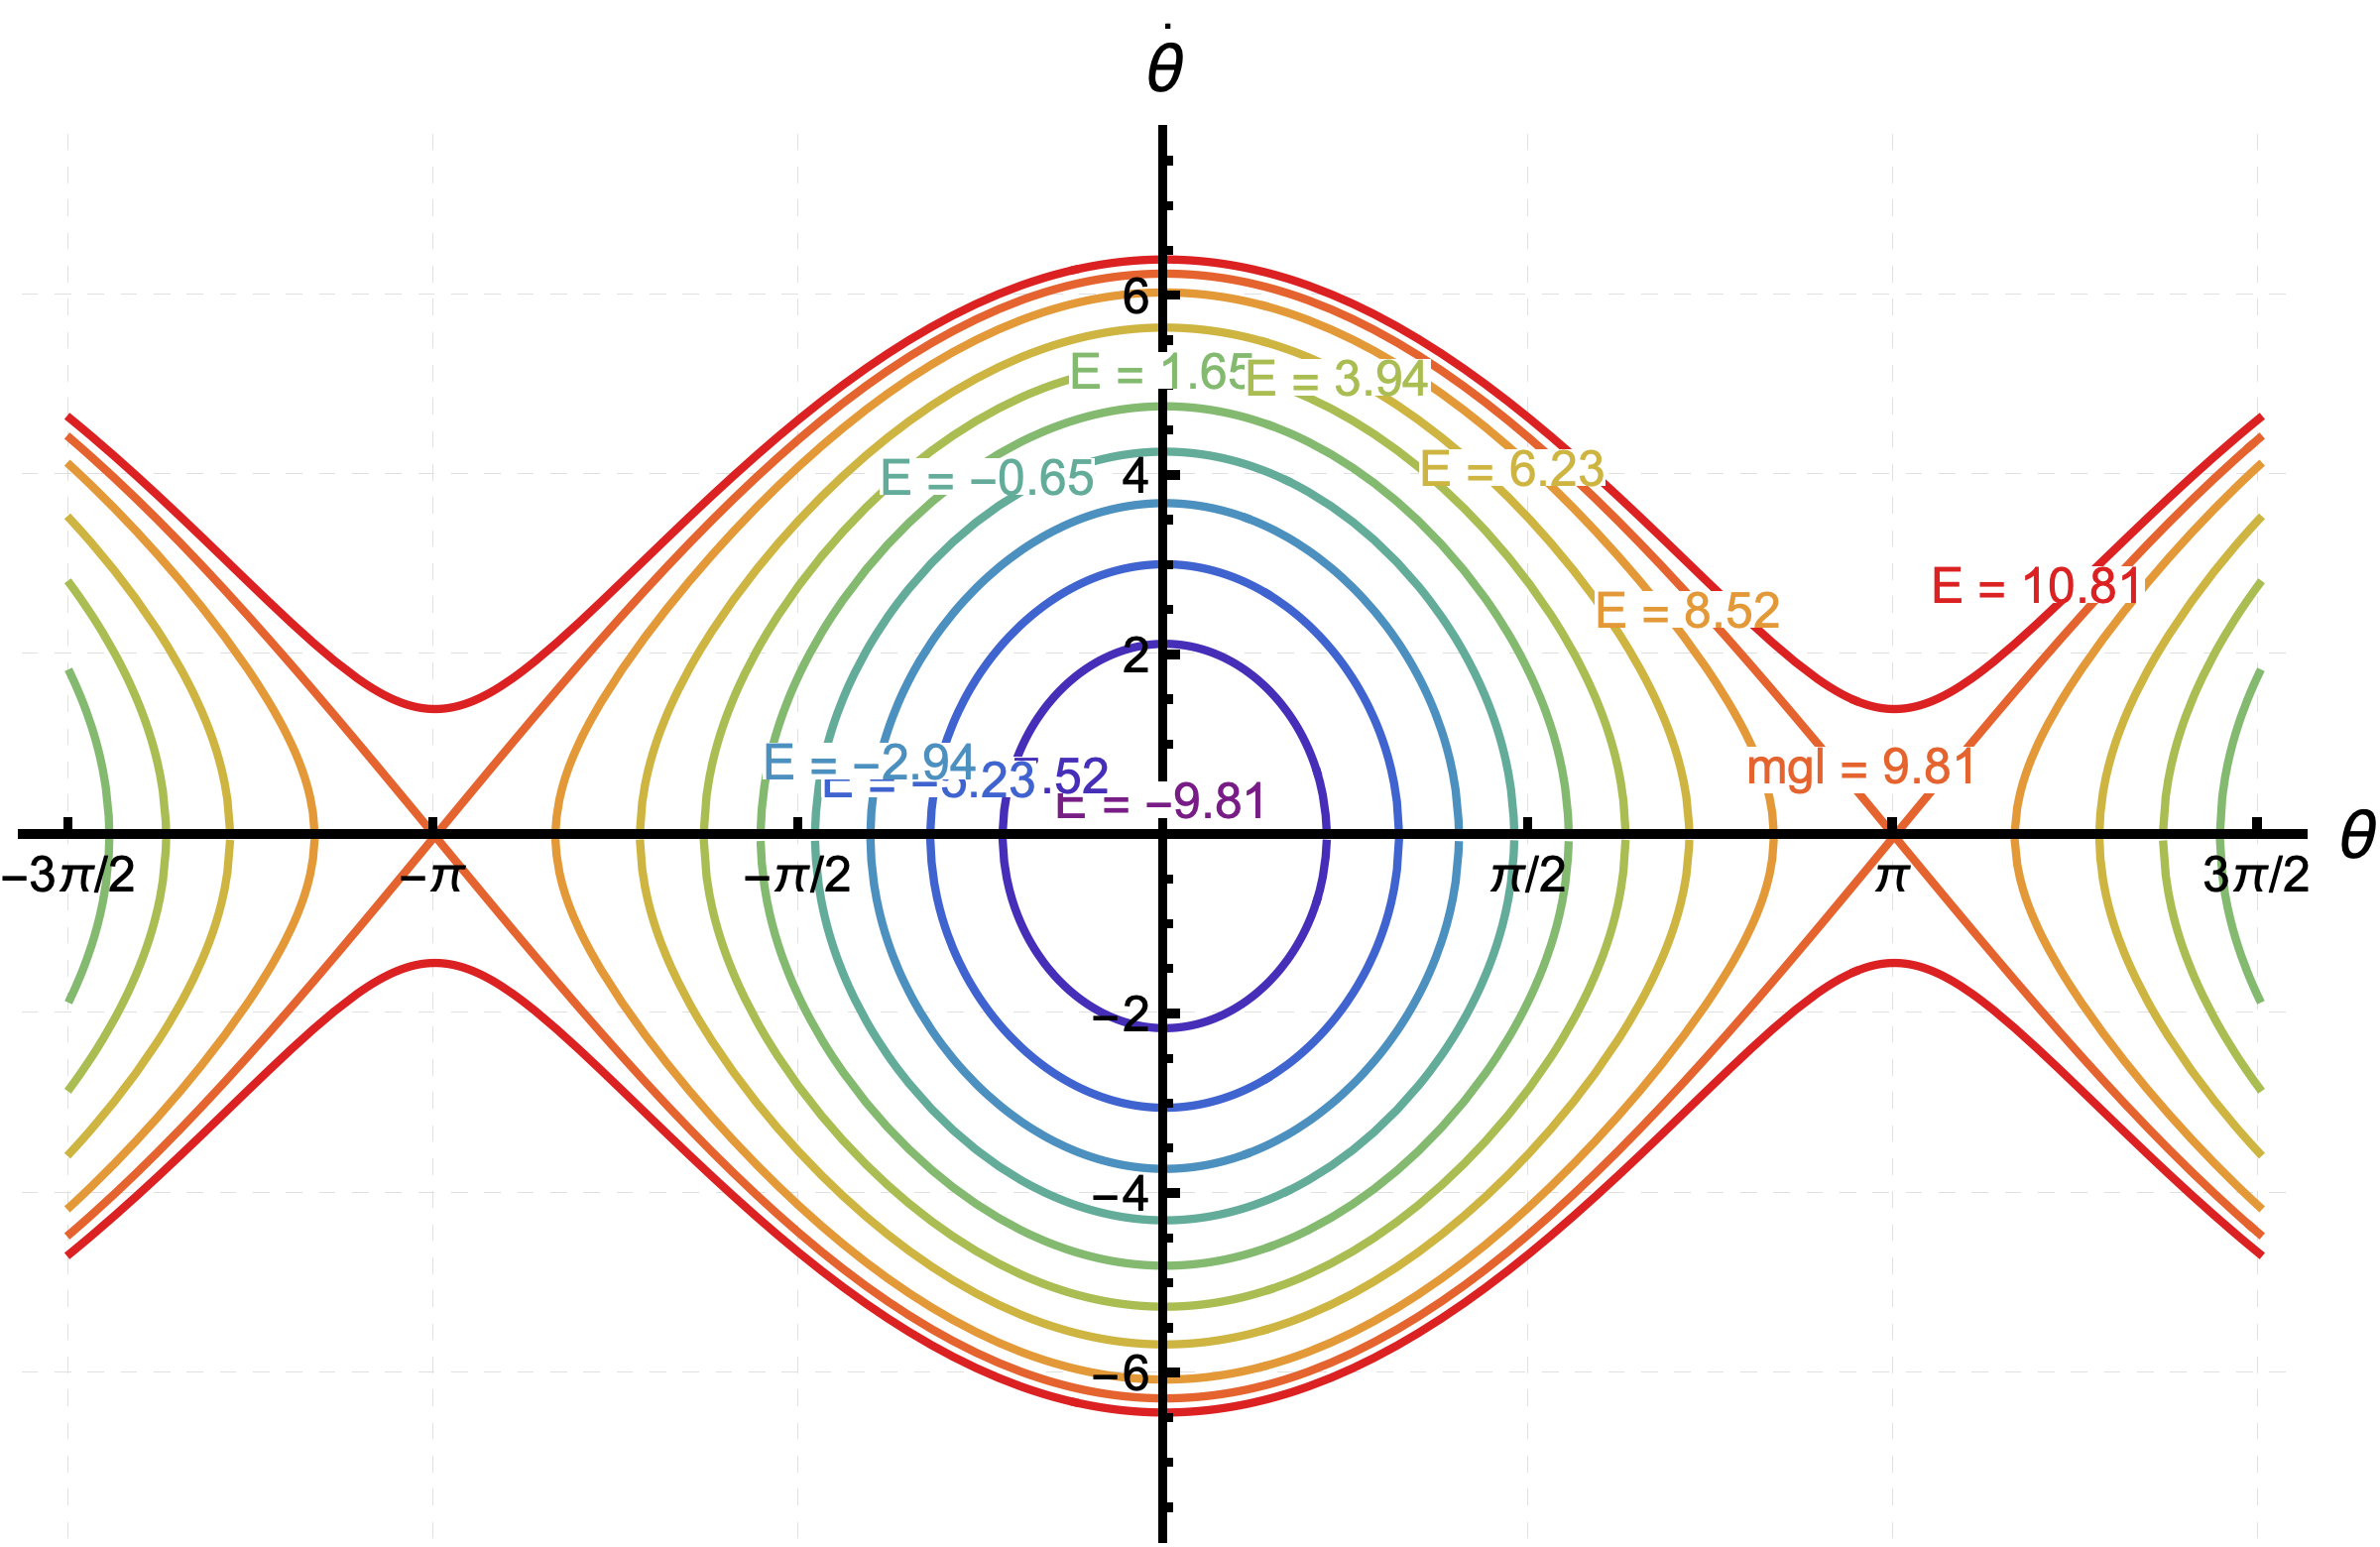
\includegraphics[scale=0.6]{immagini/grafico_pendolo.png}
\end{center}

Si può notare che se il livello energetico è basso sono permessi solo stati con
\(\theta\) piccola e che, assieme a \(\dot{\theta}\), siano confinati tra un
valore minimo e uno massimo, cioè curve chiuse.

Questo corrisponde a far oscillare il pendolo con un angolo massimo inferiore
a \(\pi\).

Per
\[
\theta=\pi,
\qquad
\dot{\theta}=0,
\]
si ha
\[
E=mg\ell
\]
e quindi
\[
1=
\frac{m\ell^2}{4mg}\dot{\theta}^{\,2}
-
\frac{(\theta-\pi)^2}{4}.
\]

È l'iperbole degenere gialla con centro \(\theta=\pi\).
\(\theta=\pi\) è l'angolo minimo per cui le curve si aprono. Vedremo come
questo è legato alla stabilità degli stati di equilibrio.

Nel piano delle fasi, per
\[
\theta\ll 1,
\]
la curva del moto del pendolo è molto simile a quella dell'oscillatore
armonico. Proviamo a caratterizzare in modo analitico quanto simile.

Oscillatore armonico:
\[
m\ddot{x}=-kx.
\]

Pendolo:
\[
m\ell^2\ddot{\theta}
=
-mg\ell\sin\theta.
\]
Per
\[
\theta\ll 1
\]
si ha
\[
\sin\theta\simeq \theta,
\]
quindi
\[
m\ell^2\ddot{\theta}
=
-mg\ell\theta.
\]

Di conseguenza
\[
\left\{
\begin{array}{l}
\theta(t)=A\cos(\omega t+\varphi),\\[1mm]
\dot{\theta}(t)=-A\omega\sin(\omega t+\varphi),
\end{array}
\right.
\qquad
\omega=\sqrt{\dfrac{g}{\ell}}.
\]

Ovvero, per
\[
\theta\ll 1,
\]
il moto è esattamente un moto armonico.

Si dimostra facilmente che le configurazioni di equilibrio del pendolo sono
\[
\theta_1=0,
\qquad
\theta_2=\pi.
\]
\end{example}



\section{Stabilità delle configurazioni di equilibrio}

Consideriamo un sistema ad un grado di libertà definito dalla coordinata libera
\[
q(t).
\]
All'equilibrio si ha
\[
\underline{f}\cdot \delta\underline{x}
=
\underline{f}\cdot
\frac{\partial \underline{x}}{\partial q}\,\delta q
=
0
\qquad \Longrightarrow \qquad
\underline{f}\cdot
\frac{\partial \underline{x}}{\partial q}
=
0.
\]

Ottengo una configurazione \(\hat{q}\). Vogliamo caratterizzare la
stabilità di questa configurazione.

\begin{example}{}[Pendolo]
Consideriamo il pendolo classico. Poniamo
\[
q=\theta.
\]
Le configurazioni di equilibrio sono
\[
\theta_1=0,
\qquad
\theta_2=\pi.
\]


Euristicamente, \(\theta=0\) è una configurazione d'equilibrio stabile perché,
se ho una condizione iniziale del moto ``vicina'', nel moto resta ``vicina'' a
\(\theta=0\).

Se invece \(\theta=\pi\), è una configurazione di equilibrio instabile perché,
se ho una condizione iniziale del moto ``vicina'', nel moto si allontana da
\(\theta=\pi\).
\end{example}

Formalmente diamo la seguente definizione di \textbf{stabilità}.
\begin{definition}{}
Sia \(\underline{q}(t)\) il moto di un sistema meccanico e sia \(\hat{\underline{q}}\) una configurazione di equilibrio.

La configurazione \(\hat{\underline{q}}\) è di equilibrio stabile se
\[
\forall \varepsilon>0\ \exists \delta>0
\]
tale che, per ogni \(\underline{q}\),
\[
\left|\hat{\underline{q}}-\underline{q}(0)\right|<\delta,
\qquad
\left|\dot{\underline{q}}(0)\right|<\delta
\ \Longrightarrow\
\left|\underline{q}(t)-\hat{\underline{q}}\right|<\varepsilon
\qquad \forall t>0.
\]
\end{definition}
Se
\[
\underline{q}=(q_1,q_2),
\]
si può visualizzare la definizione nel seguente modo:

\begin{center}
\begin{tikzpicture}[x=1cm,y=1cm,>=Latex]
    % assi
    \draw[->, line width=0.9pt] (0,0) -- (5.7,0) node[right] {$q_1$};
    \draw[->, line width=0.9pt] (0,0) -- (0,4.1) node[above] {$q_2$};

    % centro
    \coordinate (Q) at (3.2,2.2);
    \fill (Q) circle (1.2pt);

    % tacche sugli assi
    \draw[line width=0.8pt] (3.2,-0.08) -- (3.2,0.08);
    \draw[line width=0.8pt] (-0.08,2.2) -- (0.08,2.2);

    % etichette assi corrispondenti
    \node[below] at (3.2,-0.1) {$\hat{q}_1$};
    \node[left] at (-0.05,2.2) {$\hat{q}_2$};

    % palle
    \draw[red, dashed, line width=0.9pt] (Q) circle (0.65);
    \draw[green!60!black, dashed, line width=0.9pt] (Q) circle (1.15);

    % freccia delta
    \draw[->, red, line width=0.9pt] (Q) -- ++(135:0.65);
    \node[red, above left] at ($(Q)+(135:0.38)$) {$\delta$};

    % freccia epsilon
    \draw[->, green!60!black, line width=0.9pt] (Q) -- ++(-35:1.15);
    \node[green!60!black, right] at ($(Q)+(-35:0.72)$) {$\varepsilon$};

    % etichetta centro
    \node[right] at ($(Q)+(0.12,0.08)$) {$\hat{\underline{q}}$};
\end{tikzpicture}
\end{center}

Se
\[
\underline{q}(0)\in B_\delta(\hat{\underline{q}})
\quad\Longrightarrow\quad
\underline{q}(t)\in B_\varepsilon(\hat{\underline{q}})
\qquad \forall t>0.
\]



La definizione di configurazione di equilibrio stabile è complicata da usare
nella pratica. Ma per forze conservative vale il teorema di Dirichlet.

\begin{theorem}{}[Dirichlet]
Se \(\hat{\underline{q}}\) è un minimo locale stretto di \(V(\underline{q})\),
allora \(\hat{\underline{q}}\) è una configurazione d'equilibrio stabile per il
sistema.
\end{theorem}

\begin{proof}
Sia
\[
E(\underline{q},\dot{\underline{q}})
=
T(\underline{q} , \dot{\underline{q}})+V(\underline{q})
\]
l'energia totale del sistema. Poiché il sistema è conservativo si ha che
\[
E(\underline{q}(t),\dot{\underline{q}}(t))=\text{cost.}
\qquad \forall t.
\]

Inoltre
\[
T(\underline{q} , \dot{\underline{q}})\geq 0,
\qquad
T(\underline{q} , \dot{\underline{q}})=0
\Longleftrightarrow
\dot{\underline{q}}=\underline{0}.
\]

Poiché \(\hat{\underline{q}}\) è un minimo locale stretto di \(V\),
fissato \(\varepsilon\) sufficientemente piccolo, si ha che
\[
\forall \underline{q}\in \partial B_\varepsilon
(\hat{\underline{q}})
\qquad
V(\underline{q})>V(\hat{\underline{q}}).
\]

Inoltre \(\partial B_\varepsilon(\hat{\underline{q}})\) è un compatto e
la funzione
\[
V(\underline{q})-V(\hat{\underline{q}})
\]
è continua su \(\partial B_\varepsilon(\hat{\underline{q}})\) ed inoltre
strettamente positiva. Per il teorema di Weierstrass ammette minimo
\(m_\varepsilon>0\). Allora
\[
\forall \underline{q}\in \partial B_\varepsilon(\hat{\underline{q}})
\qquad
V(\underline{q})-V(\hat{\underline{q}})\geq m_\varepsilon
\]
cioè
\[
V(\underline{q})\geq m_\varepsilon+V(\hat{\underline{q}}).
\]

Abbiamo trovato che su \(\partial B_\varepsilon(\hat{\underline{q}})\)
\(V\) non può scendere al di sotto del valore di \(V\) in
\(\hat{\underline{q}}\) maggiorato di una costante positiva.

Ricordiamo ora che
\[
E(\underline{q},\dot{\underline{q}})
\]
è continua e in particolare lo è in
\[
(\hat{\underline{q}},\underline{0}),
\]
punto di equilibrio. Allora, fissato \(m_\varepsilon>0\) come sopra,
\[
\exists \ell>0
\]
tale che
\[
\left|
(\hat{\underline{q}},\underline{0})
-
(\underline{q}(0),\dot{\underline{q}}(0))
\right|<\ell
\]
implica
\[
\left|
E(\underline{q}(0),\dot{\underline{q}}(0))
-
E(\hat{\underline{q}},\underline{0})
\right|
=
\left|
E(\underline{q}(0),\dot{\underline{q}}(0))
-
V(\hat{\underline{q}})
\right|
<m_\varepsilon.
\]

Possiamo ripartire la distanza da
\[
(\hat{\underline{q}},\underline{0})
\]
sulle \(2\) componenti e dire che
\[
\exists \delta^*>0
\]
tale che
\[
|\hat{\underline{q}}-\underline{q}(0)|<\delta^*,
\qquad
|\dot{\underline{q}}(0)|<\delta^*
\]
implica
\[
\left|
E(\underline{q}(0),\dot{\underline{q}}(0))
-
V(\hat{\underline{q}})
\right|
<m_\varepsilon.
\]
Quindi
\[
E(\underline{q}(0),\dot{\underline{q}}(0))
<
m_\varepsilon+V(\hat{\underline{q}}).
\]

La condizione vale anche per
\[
\delta=\min\{\delta^*,\varepsilon\}.
\]

Considero quindi \(\underline{q}(t)\) tale che
\[
|\underline{q}(0)-\hat{\underline{q}}|<\delta,
\qquad
|\dot{\underline{q}}(0)|<\delta,
\]
ovvero ci siamo messi in una situazione iniziale con energia totale minore
dell'energia potenziale minima su
\(\partial B_\varepsilon(\hat{\underline{q}})\) e con posizione iniziale
\[
\underline{q}(0)\in B_\varepsilon(\hat{\underline{q}}).
\]

Supponiamo per assurdo che esista un istante \(t_1\geq 0\) tale che
\[
\underline{q}(t_1)\notin B_\varepsilon(\hat{\underline{q}}),
\]
ovvero
\[
|\underline{q}(t_1)-\hat{\underline{q}}|\geq \varepsilon.
\]

Per continuità di \(\underline{q}(t)\) deve esistere
\[
0\leq t^*\leq t_1
\]
tale che
\[
\underline{q}(t^*)\in \partial B_\varepsilon(\hat{\underline{q}}).
\]

Analizziamo il bilancio energetico all'istante \(t^*\):
\[
E(\underline{q}(t^*),\dot{\underline{q}}(t^*))
=
T(\dot{\underline{q}}(t^*))
+
V(\underline{q}(t^*))
\geq
V(\hat{\underline{q}})+m_\varepsilon
+
T(\dot{\underline{q}}(t^*))
\geq
V(\hat{\underline{q}})+m_\varepsilon.
\]

D'altra parte
\[
E(\underline{q}(t^*),\dot{\underline{q}}(t^*))
<
m_\varepsilon+V(\hat{\underline{q}}).
\]

Abbiamo trovato che
\[
E(\underline{q}(t^*),\dot{\underline{q}}(t^*))
\]
deve essere maggiore o uguale e minore di una quantità, che è un assurdo.

Allora
\[
|\underline{q}(0)-\hat{\underline{q}}|<\delta,
\qquad
|\dot{\underline{q}}(0)|<\delta
\]
implica
\[
|\underline{q}(t)-\hat{\underline{q}}|<\varepsilon
\qquad
\forall t>0.
\]
Ovvero \(\hat{\underline{q}}\) è stabile.
\end{proof}

Possiamo quindi individuare i punti di equilibrio risolvendo $\nabla V(\underline{q}) = 0$ e caratterizzando la loro stabilità studiando il segno degli autovalori della matrice hessiana $H_V(\underline{q})$.
\begin{example}{}
    Riconsideriamo l'esempio dello scorso capitolo con le stesse ipotesi e studiamo la stabilità delle configurazioni di equilibrio.

    \begin{center}
    \begin{tikzpicture}[
    x=1cm,
    y=1cm,
    >=Latex,
    line cap=round,
    line join=round,
    every node/.style={font=\small}
]

% Parametri
\def\R{1.55}

% Coordinate
\coordinate (O) at (0,0);
\coordinate (A) at (0,3.45);
\coordinate (G) at (7.20,\R);
\coordinate (C) at (7.20,0);
\coordinate (Top) at ($(G)+(0,\R)$);
\coordinate (B) at ($(A)!0.42!(G)$);

% Assi
\draw[black, line width=1.4pt, ->] (0,0) -- (10.2,0) node[below right] {$x$};
\draw[black, line width=1.4pt, ->] (0,0) -- (0,4.2) node[above left] {$y$};

% Parete verticale
\draw[black, line width=2pt] (0,0) -- (0,4.05);

% Origine
\node[below left] at (O) {$O$};

% Riferimento centrato in O
\draw[orange!85!black, line width=1.4pt, ->] (O) -- ++(0.95,0);
\draw[orange!85!black, line width=1.4pt, ->] (O) -- ++(0,0.95);
\node[orange!85!black, below] at ($(O)+(0.48,0)$) {$\underline{\imath}$};
\node[orange!85!black, left] at ($(O)+(0,0.48)$) {$\underline{\jmath}$};

\draw[orange!85!black, line width=1.2pt] (-0.45,0.18) circle (0.18);
\fill[orange!85!black] (-0.45,0.18) circle (0.03);
\node[orange!85!black, left] at (-0.62,0.62) {$\underline{k}$};

% Sbarrette verticali attaccate all'asse y
\draw[black, line width=1.6pt] (0,3.14) -- (0,3.56);
\draw[black, line width=1.6pt] (0.12,3.14) -- (0.12,3.56);

% Punto A
\node[left] at (A) {$A$};

% Asta
\draw[black, line width=1.8pt] (A) -- (G);

% Punto B
\fill[red] (B) circle (2.8pt);
\node[above] at (B) {$B$};

% Etichetta asta
\node[above right] at ($(B)!0.52!(G)$) {$l,m$};

% Angolo theta
\draw[black, line width=1.1pt]
($(A)+(0,-0.78)$) arc[start angle=-90,end angle=-14.5,radius=0.78];
\node at ($(A)+(0.72,-0.87)$) {$\theta$};

% Freccia verde in A
\draw[green!55!black, line width=1.4pt, ->] ($(A)$) -- ++(1.80,0);
\node[green!55!black, above] at ($(A)+(1.25,0.20)$) {$\underline{\psi}$};

% Molla attaccata all'asse y
\draw[black, line width=1.4pt, smooth, samples=240, domain=0:7.02]
plot (\x,{1.55 + 0.10*sin(900*\x)});

% Ruota
\draw[black, line width=1.8pt] (G) circle (\R);

% Punto C
\node[below] at (C) {$C$};

% Centro G
\filldraw[white, draw=black, line width=1.2pt] (G) circle (0.09);
\node[above left] at ($(G)+(-0.10,0.08)$) {$G$};

% Etichetta M,R
\node[above right] at ($(Top)+(0.95,-0.05)$) {$M,R$};

% Raggi tratteggiati
\draw[black, dashed, line width=1.1pt] (Top) -- (G);
\draw[black, dashed, line width=1.1pt] (G) -- ++(0.95,1.00);

% Angolo phi
\draw[black, line width=1.0pt, ->]
($(G)+(0,0.58)$) arc[start angle=90,end angle=46,radius=0.58];
\node at ($(G)+(0.47,0.92)$) {$\varphi$};

% Forza mg in B
\draw[red!85!black, line width=1.5pt, ->] (B) -- ++(0,-1.15);
\node[red!85!black, left] at ($(B)+(0.10,-0.70)$) {$m\underline{g}$};

% Forza Mg in G
\draw[red!85!black, line width=1.5pt, ->] (G) -- ++(0,-1.05);
\node[red!85!black, right] at ($(G)+(0.52,-0.62)$) {$M\underline{g}$};

% Forza elastica
\draw[red!85!black, line width=1.5pt, ->] (G) -- ++(-1.25,0);
\node[red!85!black, below] at ($(G)+(-0.82,-0.12)$) {$-k\,\underline{x}_G$};

% Assi verdi vicino a C
\draw[green!55!black, line width=1.4pt, ->] ($(C)+(0.18,0)$) -- ++(1.90,0);
\draw[green!55!black, line width=1.4pt, ->] ($(C)+(0.18,0)$) -- ++(0,0.95);
\node[green!55!black, right] at ($(C)+(2.10,0)$) {$\underline{\xi}_x$};
\node[green!55!black, right] at ($(C)+(0.22,0.58)$) {$\underline{\xi}_y$};

\end{tikzpicture}
  \end{center}


  Studiamo la stabilità delle configurazioni d'equilibrio. Il potenziale
\(V(\theta)\) è
\[
V
=
\frac{kx_G^2}{2}
+
mg\left(R+\frac{\ell}{2}\cos\theta\right)
+
MgR
=
\frac{k}{2}\ell^2\sin^2\theta
+
mg\left(R+\frac{\ell}{2}\cos\theta\right)
+
MgR.
\]

Allora
\[
\nabla V
=
\frac{dV}{d\theta}
=
2\frac{k}{2}\ell^2\sin\theta\cos\theta
-
mg\frac{\ell}{2}\sin\theta
=
0,
\]
cioè
\[
k\ell^2\sin\theta\cos\theta
-
mg\frac{\ell}{2}\sin\theta
=
0.
\]

Quindi
\[
\theta_1=0,
\qquad
\theta_2=\pi,
\qquad
\cos\theta_{3,4}
=
\frac{mg}{2k\ell}
\quad
\text{se}
\quad
\frac{mg}{2k\ell}\leq 1.
\]

Sono le configurazioni d'equilibrio.

Calcoliamo la derivata seconda, cioè l'hessiana:
\[
\frac{d^2V}{d\theta^2}
=
k\ell^2\cos^2\theta
-
k\ell^2\sin^2\theta
-
mg\frac{\ell}{2}\cos\theta.
\]

Valuto nelle configurazioni di equilibrio:
\[
\frac{d^2V}{d\theta^2}(0)
=
k\ell^2
-
mg\frac{\ell}{2}.
\]
Quindi è stabile se
\[
k\ell^2>mg\frac{\ell}{2}
\Longleftrightarrow
2k\ell>mg
\Longleftrightarrow
1>\frac{mg}{2k\ell}.
\]

Inoltre
\[
\frac{d^2V}{d\theta^2}(\pi)
=
k\ell^2
+
mg\frac{\ell}{2}
>
0,
\]
quindi è sempre stabile.

Infine
\[
\left.
\frac{d^2V}{d\theta^2}(\theta_3,\theta_4)
=
k\ell^2\cos^2\theta
-
k\ell^2(1-\cos^2\theta)
-
mg\frac{\ell}{2}\cos\theta
\right|_{\theta_3,\theta_4}
\]
\[
=
\frac{(mg)^2}{4k}
-
k\ell^2
>
0.
\]
Dunque
\[
(mg)^2>4k^2\ell^2
\Longleftrightarrow
mg>2k\ell
\Longleftrightarrow
1<
\frac{mg}{2k\ell}.
\]









  \begin{center}
  \begin{tikzpicture}[scale=1, line cap=round, line join=round, >=Latex]

%======================
% Disegno 1
%======================
\begin{scope}[shift={(0,0)}]
    \node at (0,3.35) {$\theta_1=0$};

    % piano
    \draw[line width=0.9pt] (-1.7,0) -- (1.7,0);

    % disco
    \draw[line width=1pt] (0,1) circle (1);

    % asta verticale
    \draw[line width=1pt] (0,1) -- (0,2.85);

    % punto A e guida
    \fill (0,2.15) circle (1.2pt);
    \node[right] at (0,2.15) {$A$};
    \draw[line width=0.8pt] (-0.13,1.90) -- (-0.13,2.40);
    \draw[line width=0.8pt] ( 0.13,1.90) -- ( 0.13,2.40);
\end{scope}

%======================
% Disegno 2
%======================
\begin{scope}[shift={(5.6,0)}]
    \node at (0,3.35) {$\theta_2=\pi$};

    % piano
    \draw[line width=0.9pt] (-1.7,0) -- (1.7,0);

    % disco
    \draw[line width=1pt] (0,1) circle (1);

    % asta verticale verso il basso
    \draw[line width=1pt] (0,1) -- (0,-1.05);

    % punto A e guida
    \fill (0,-0.38) circle (1.2pt);
    \node[right] at (0,-0.38) {$A$};
    \draw[line width=0.8pt] (-0.13,-0.63) -- (-0.13,-0.13);
    \draw[line width=0.8pt] ( 0.13,-0.63) -- ( 0.13,-0.13);
\end{scope}

%======================
% Disegno 3
%======================
\begin{scope}[shift={(12.4,0)}]
    \node at (0,3.35) {$\theta_3,\theta_4$};

    % piano con freccia
    \draw[line width=0.9pt, ->] (-3.3,0) -- (4.2,0);

    % asse verticale centrale
    \draw[line width=1pt] (0,-1.4) -- (0,2.95);

    % dischi
    \draw[line width=1pt] (-1.7,1) circle (1);
    \draw[line width=1pt] ( 1.7,1) circle (1);

    % centri dei dischi
    \coordinate (GL) at (-1.7,1);
    \coordinate (GR) at ( 1.7,1);
    \coordinate (A)  at (0,2.18);

    % punto A e guida
    \fill (A) circle (1.2pt);
    \node[right] at (A) {$A$};
    \draw[line width=0.8pt] (-0.13,1.92) -- (-0.13,2.42);
    \draw[line width=0.8pt] ( 0.13,1.92) -- ( 0.13,2.42);

    % aste inclinate che partono dai centri delle circonferenze
    \draw[line width=1pt] (GL) -- (A);
    \draw[line width=1pt] (GR) -- (A);

    % molla orizzontale tra i due centri
    \draw[line width=1pt] (-1.7,1) -- (-1.25,1);

    \draw[line width=1pt, smooth, samples=100, domain=-1.25:-0.15]
        plot (\x,{1 + 0.07*sin((\x+1.25)/1.10*1080)});

    \fill (0,1) circle (1.2pt);

    \draw[line width=1pt, smooth, samples=100, domain=0.15:1.25]
        plot (\x,{1 + 0.07*sin((\x-0.15)/1.10*1080)});

    \draw[line width=1pt] (1.25,1) -- (1.7,1);
\end{scope}

\end{tikzpicture}
\end{center}


\[
\begin{array}{ll}
\bullet & \theta_1=0
\quad \text{esiste sempre ed è stabile per }
\dfrac{mg}{2k\ell}<1,
\\[4mm]
\bullet & \theta_2=\pi
\quad \text{esiste ed è stabile sempre},
\\[4mm]
\bullet & \theta_3,\theta_4
\quad \text{esistono per }
\dfrac{mg}{2k\ell}\leq 1
\quad \text{e sono stabili per }
\dfrac{mg}{2k\ell}>1.
\end{array}
\]

Ovvero:
\[
\begin{array}{ll}
\bullet &
\dfrac{mg}{2k\ell}>1
\quad \Longrightarrow \quad
\exists\,\theta_1,\theta_2,
\\[3mm]
&
\theta_1 \text{ instabile},
\qquad
\theta_2 \text{ stabile};
\\[6mm]
\bullet &
\dfrac{mg}{2k\ell}<1
\quad \Longrightarrow \quad
\exists\,\theta_1,\theta_2,\theta_3,\theta_4,
\\[3mm]
&
\theta_1 \text{ stabile},
\qquad
\theta_2 \text{ stabile},
\\[2mm]
&
\theta_3,\theta_4 \text{ instabili}.
\end{array}
\]
\end{example}
